\newpage
\section{Ứng dụng của CLIP}
\subsection{Ứng dụng CLIP trong truy vấn Ảnh - Văn bản}

\paragraph{}{Mô hình CLIP (Contrastive Language-Image Pretraining) do OpenAI phát triển là một bước tiến quan trọng trong việc xây dựng hệ thống truy vấn đa phương thức, cho phép tìm kiếm chéo giữa ảnh và văn bản. Với CLIP, người dùng có thể nhập truy vấn văn bản để tìm ảnh phù hợp hoặc nhập ảnh để truy xuất mô tả văn bản gần nhất.}

\paragraph{}{Ví dụ: Truy vấn văn bản “người đàn ông đeo kính” có thể giúp hệ thống tìm ra các hình ảnh tương ứng trong tập dữ liệu. CLIP được ứng dụng rộng rãi trong các lĩnh vực như tìm kiếm hình ảnh, gợi ý nội dung, kiểm duyệt nội dung tự động, và nhiều tác vụ liên quan đến AI thị giác.
}

\subsubsection{Bộ dữ liệu COCO 2017}
\paragraph{} {Nguồn dữ liệu: \url{https://www.kaggle.com/datasets/awsaf49/coco-2017-dataset/data}

\paragraph{}{Bộ dữ liệu COCO (Common Objects in Context) được sử dụng phổ biến trong huấn luyện và đánh giá các mô hình học sâu trong thị giác máy tính, bao gồm cả mô hình CLIP. COCO cung cấp ảnh gắn nhãn kèm theo mô tả ngôn ngữ tự nhiên (caption), rất phù hợp cho bài toán truy vấn ảnh-văn bản.}

\begin{itemize}
    \item \textbf{Train2017:} Khoảng 118.000 ảnh gán nhãn dùng để huấn luyện.
    \item \textbf{Val2017:} 5.000 ảnh dùng để đánh giá mô hình.
    \item \textbf{Test2017:} 41.000 ảnh (không có nhãn công khai).
    \item \textbf{Caption:} Mỗi ảnh đi kèm trung bình 5 mô tả ngắn do con người viết.
    \item \textbf{Định dạng:} Ảnh `.jpg` và nhãn định dạng `.json` theo chuẩn COCO.
\end{itemize}

COCO là bộ dữ liệu tiêu chuẩn được nhiều mô hình như CLIP, BLIP, ViLT, Flamingo sử dụng trong huấn luyện và đánh giá.

\subsubsection{Thực hiện Truy vấn Ảnh - Văn bản với CLIP}

Do việc huấn luyện mô hình từ đầu trên bộ dữ liệu lớn tốn kém tài nguyên (GPU, thời gian), ta sử dụng mô hình CLIP ViT-B/32 đã được huấn luyện sẵn bởi OpenAI. Các bước thực hiện như sau:

\begin{itemize}
    \item \textbf{Bước 1:} Nạp mô hình CLIP ViT-B/32 từ thư viện \texttt{clip} của OpenAI.
    \item \textbf{Bước 2:} Tiền xử lý ảnh và văn bản đầu vào (resize, chuẩn hóa, token hóa).
    \item \textbf{Bước 3:} Trích xuất vector đặc trưng (embedding) từ cả ảnh và văn bản.
    \item \textbf{Bước 4:} Tính độ tương đồng cosine giữa các vector để xác định cặp gần nhất.
    \item \textbf{Bước 5:} Truy xuất ảnh hoặc văn bản tương ứng có độ tương đồng cao nhất.
\end{itemize}

\subsubsection{Kết quả trên tập COCO Validation}

Mô hình CLIP ViT-B/32 được đánh giá trên tập \texttt{val2017} của COCO với các chỉ số truy xuất gồm:

\begin{itemize}
    \item \textbf{Recall@1:} 49.92\%
    \item \textbf{Recall@5:} 74.94\%
    \item \textbf{Recall@10:} 83.24\%
\end{itemize}

\textbf{Nhận xét:}
\begin{itemize}
    \item CLIP cho kết quả tốt ở Recall@10 (trên 83\%), cho thấy khả năng bao phủ cao.
    \item Recall@1 còn hạn chế ($\sim$ 50\%) – mô hình có thể nhầm lẫn khi các caption có ngữ nghĩa gần nhau.
    \item Phù hợp với các ứng dụng cần truy xuất nhiều kết quả để chọn lọc (top-5, top-10).
\end{itemize}

\subsubsection{Ví dụ minh hoạ kết quả truy vấn}

\paragraph{}{Hình dưới đây minh hoạ một truy vấn văn bản và kết quả truy xuất ảnh tương ứng.}

\begin{figure}[H]
    \centering
    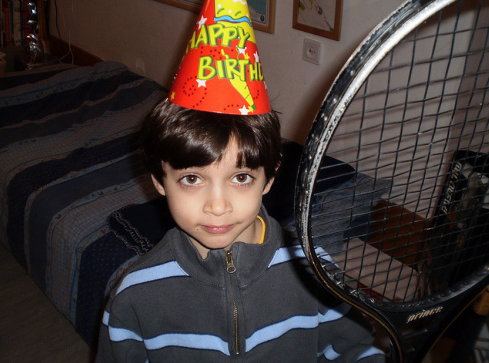
\includegraphics[width=0.6\linewidth]{img/05-imagecaption.png} % Thay bằng đường dẫn thực tế
    \caption{\textit{Ảnh minh hoạ kết quả truy vấn từ văn bản}}
\end{figure}

\textbf{Truy vấn văn bản:}
\begin{itemize}
    \item “A boy in birthday hat holding a tennis racket”
    \item “A boy swinging a tennis racket at a ball on a court.”
\end{itemize}

\textbf{Caption gốc của ảnh:}
\begin{itemize}
    \item “A boy in birthday hat holding a tennis racket"
    \item "A young boy in a birthday hat holds a tennis racquet”
\end{itemize}

\subsection{Ứng dụng của CLIP để phân biệt khuôn mặt, từ đó phát triển tác vụ nhận diện khuôn mặt người.}
\paragraph{}{CLIP (Contrastive Language–Image Pretraining) là mô hình được huấn luyện trên hàng trăm triệu cặp dữ liệu văn bản và hình ảnh để học mối liên hệ giữa chúng. Mặc dù không được thiết kế chuyên biệt cho nhận diện khuôn mặt, CLIP có khả năng biểu diễn hình ảnh mạnh mẽ, cho phép ứng dụng hiệu quả trong các bài toán phân loại và nhận diện khuôn mặt.}

\subsubsection{Mục tiêu}
\begin{itemize}
    \item Mã hóa ảnh khuôn mặt thành vector đặc trưng (embedding).
    \item Dự đoán và phân biệt khuôn mặt bằng cách so sánh độ tương đồng giữa các embedding.
\end{itemize}

\subsubsection{Dữ liệu}

\paragraph{}{Nguồn dữ liệu: \url{https://www.kaggle.com/datasets/stoicstatic/face-recognition-dataset}}
\paragraph{} {Bộ dữ liệu được xây dựng dựa trên tập \textbf{Labeled Faces in the Wild} với ảnh JPEG của những người nổi tiếng, mỗi ảnh có kích thước 250x250. Mỗi thư mục trong dataset đại diện cho một người nổi tiếng, chứa từ 2 đến 50 ảnh khuôn mặt.}

\begin{figure}[h!]
    \centering
    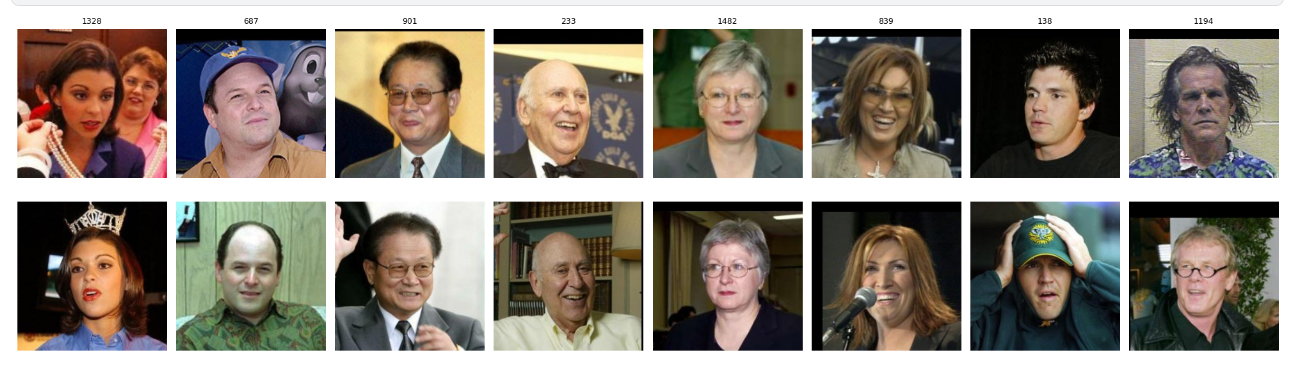
\includegraphics[width=1\textwidth]{img/05-Face.png}
    \caption{Các khuôn mặt trong tập dữ liệu nhận diện.}
    \label{fig:example_face}
\end{figure}


\paragraph{Xử lý dữ liệu}
\begin{enumerate}
    \item Áp dụng kỹ thuật tăng cường dữ liệu (augmentation) để cân bằng số lượng ảnh giữa các lớp.
    \item Chia dữ liệu thành tập huấn luyện (Train) và kiểm tra (Test).
    \item Tạo \texttt{Dataloader} cho việc huấn luyện theo cặp ảnh.
\end{enumerate}

\subsubsection{Xây dựng mô hình}

\paragraph{}{Chúng tôi sử dụng kiến trúc mô hình ViT-B/32 của CLIP để rút trích đặc trưng khuôn mặt. Chúng tôi đã mô phỏng lại các lớp trong ViT-B/32 để huấn luyện nhận diện khuôn mặt bằng Contrastive Learning.}

\paragraph{}{Kiến trúc mô hình ViT-B/32 (Sử dụng lại lớp Vision Transformer)}
\begin{itemize}
    \item \textbf{Patch Embedding:} Ảnh RGB được chia thành các patch kích thước $32 \times 32$ và chuyển thành vector.
    \item \textbf{LayerNorm:} Chuẩn hóa đầu vào cho Transformer.
    \item \textbf{Transformer Encoder:} Gồm 12 khối ResidualAttentionBlock:
    \begin{itemize}
        \item Mỗi block có multi-head attention với đầu vào/ra 768 chiều.
        \item Chuẩn hóa (\texttt{ln\_1}, \texttt{ln\_2}).
        \item MLP: Linear(768 $\rightarrow$ 3072) $\rightarrow$ QuickGELU $\rightarrow$ Linear(3072 $\rightarrow$ 768).
    \end{itemize}
    \item \textbf{Output LayerNorm:} Chuẩn hóa lần cuối để lấy embedding có đầu ra 768.
\end{itemize}

\subsubsection{Huấn luyện}

\begin{itemize}
    \item Hàm mất mát: \textbf{Contrastive Loss}.
    \item Thuật toán tối ưu: \textbf{Adam}, với tốc độ học ban đầu là $1e^{-3}$.
    \item Số epoch: \textbf{3}. (Do mô hình khá phức tạp và huấn luyện rất tốn GPU nên chúng tôi chỉ mô phỏng huấn luyện qua 3 epoch để thấy được sự khác biệt.) 
    \item Dữ liệu được cung cấp dưới dạng các cặp ảnh:
    \begin{itemize}
        \item Cặp dương tính: Hai ảnh cùng người.
        \item Cặp âm tính: Hai ảnh khác người.
    \end{itemize}
\end{itemize}
\paragraph{}{Kết quả huấn luyện cho thấy loss giảm ổn định sau mỗi epoch, cho thấy mô hình học được biểu diễn đặc trưng khuôn mặt hiệu quả.}
\begin{figure}[H]
    \centering
    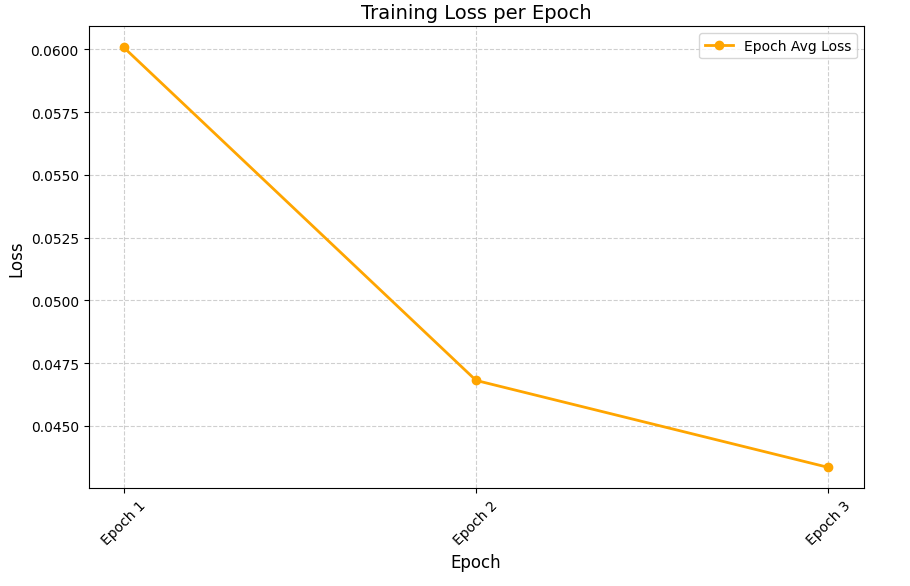
\includegraphics[width=0.7\textwidth]{img/05-loss.png} % ← thay bằng đường dẫn ảnh biểu đồ thực tế
    \caption{Biểu đồ loss theo từng epoch trong quá trình huấn luyện.}
    \label{fig:loss}
\end{figure}

\paragraph{Nhận xét}

Mô hình hiện tại mới chỉ được huấn luyện trong \textbf{3 epoch} với dữ liệu \textbf{giới hạn}, dẫn đến chất lượng embedding chưa thực sự ổn định. Cụ thể:

\begin{itemize}
    \item Các vector đặc trưng (embedding) của ảnh \textbf{cùng một người} chưa hoàn toàn hội tụ gần nhau.
    \item Các ảnh \textbf{khác người} đôi khi chưa được tách biệt rõ ràng trong không gian vector.
\end{itemize}

\vspace{0.5em}
\noindent
\textbf{Các chỉ số đánh giá mô hình:}

\begin{table}[H]
    \centering
    \renewcommand{\arraystretch}{1.3}
    \begin{tabular}{|l|c|c|}
        \hline
        \textbf{Chỉ số} & \textbf{Tập Train} & \textbf{Tập Test} \\
        \hline
        Accuracy        & 72.92\%                 & 71.65\%            \\
        Precision       & 83.56\%                 & 66.76\%            \\
        Recall          &57.06\%              & 86.24\%            \\
        F1-score        & 67.81\%               & 75,26\%            \\
        \hline
    \end{tabular}
\end{table}

\vspace{0.5em}
\noindent
\textbf{Confusion Matrix:}

\begin{figure}[H]
    \centering
    \begin{subfigure}[b]{0.48\textwidth}
        \centering
        \includegraphics[width=\textwidth]{img/05-Train.png}
        \caption{Tập Train}
    \end{subfigure}
    \hfill
    \begin{subfigure}[b]{0.48\textwidth}
        \centering
        \includegraphics[width=\textwidth]{img/05-Test.png}
        \caption{Tập Test}
    \end{subfigure}
    \caption{Ma trận nhầm lẫn trên tập train và test}
\end{figure}

\vspace{0.5em}

\noindent
\paragraph{}{Mô hình đạt Accuracy 72.92\% (train) và 71.65\% (test), cho thấy độ ổn định tương đối giữa hai tập dữ liệu. Precision giảm từ 83.56\% xuống 66.76\%, phản ánh sự xuất hiện của nhiều dự đoán dương tính sai trên tập test. Ngược lại, Recall tăng mạnh từ 57.06\% lên 86.24\%, cho thấy mô hình nhận diện hiệu quả các cặp ảnh cùng người. F1-score cũng được cải thiện, từ 67.81\% lên 75.26\%, thể hiện sự cân bằng tốt hơn giữa precision và recall. \\

Trên tập kiểm thử, mô hình bước đầu phân biệt được ảnh khuôn mặt cùng và khác người, nhưng vẫn cần tinh chỉnh thêm để tối ưu hóa hiệu suất.}

\vspace{0.5em}
\noindent
\textbf{Ví dụ minh họa trên tập test:}

\begin{figure}[H]
    \centering
    \begin{minipage}[b]{0.48\textwidth}
        \centering
        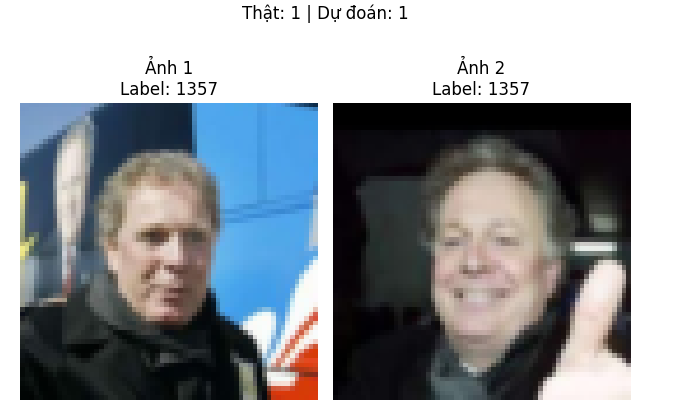
\includegraphics[width=\linewidth]{img/05-1.png}
        \caption*{Khoảng cách: 0.6384\\Thật: 0, Dự đoán: 0}
    \end{minipage}
    \hfill
    \begin{minipage}[b]{0.48\textwidth}
        \centering
        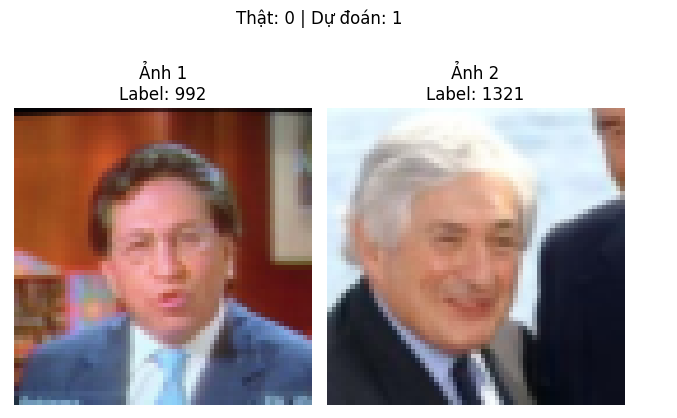
\includegraphics[width=\linewidth]{img/05-2.png}
        \caption*{Khoảng cách: 0.0605\\Thật: 1, Dự đoán: 1}
    \end{minipage}
    
    \vspace{0.5cm}
    
    \begin{minipage}[b]{0.48\textwidth}
        \centering
        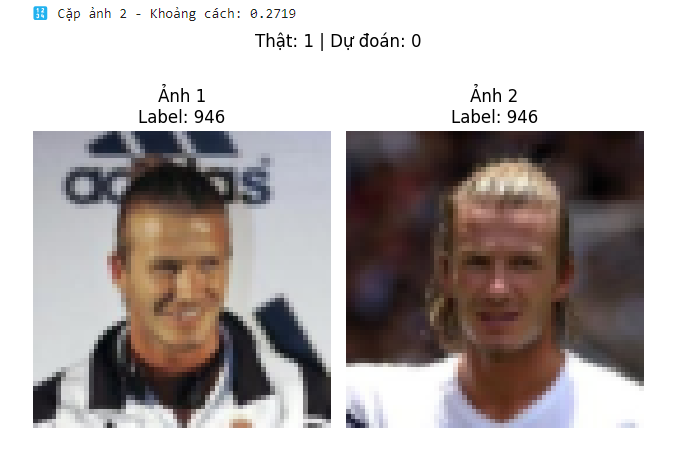
\includegraphics[width=\linewidth]{img/05-3.png}
        \caption*{Khoảng cách: 0.2719\\Thật: 1, Dự đoán: 0}
    \end{minipage}
    \hfill
    \begin{minipage}[b]{0.48\textwidth}
        \centering
        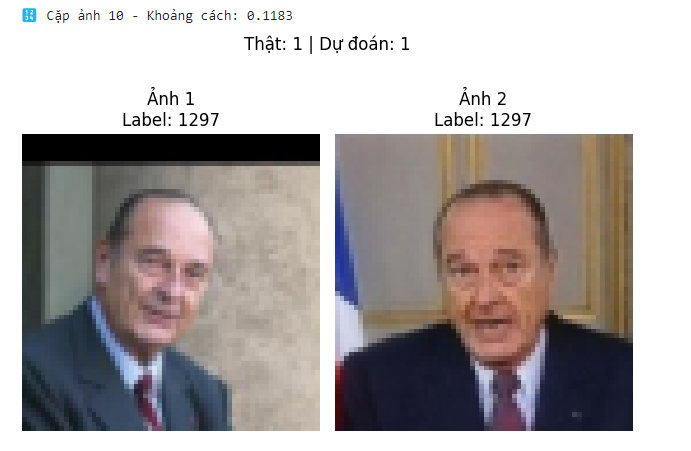
\includegraphics[width=\linewidth]{img/05-4.png}
        \caption*{Khoảng cách: 0.1183\\Thật: 1, Dự đoán: 1}
    \end{minipage}
    
    \caption{Một số dự đoán minh họa trên tập kiểm thử}
    \label{fig:comparison}
\end{figure}

\vspace{1em}
\noindent
\textbf{Kết luận:}  

Việc huấn luyện ngắn hạn đã giúp mô hình bước đầu học được biểu diễn khái quát về khuôn mặt. Tuy nhiên, để cải thiện hiệu năng, cần:

\begin{itemize}
    \item Tăng số lượng epoch huấn luyện.
    \item Bổ sung thêm dữ liệu đa dạng hơn.
\end{itemize}

\subsubsection{So sánh và đánh giá trong tác vụ nhận diện khuôn mặt}
 
\paragraph{}{Mặc dù CLIP không được thiết kế chuyên biệt cho nhiệm vụ nhận diện khuôn mặt, nhưng nó có khả năng trích xuất đặc trưng từ ảnh và so sánh với các mẫu đã biết để tìm ra ảnh có đặc trưng gần nhất. Nếu ảnh gần nhất tương ứng với một khuôn mặt đã được gán nhãn, mô hình sẽ dự đoán đó là khuôn mặt tương ứng.}

\paragraph{}{Để đánh giá hiệu quả của CLIP trong bài toán nhận diện khuôn mặt, chúng tôi tiến hành so sánh với bốn mô hình CNN tiêu biểu khác.}

\begin{table}[H]
\centering
\begin{tabular}{|c|c|c|c|c|}
\hline
\textbf{Mô hình} & Accuracy & Precision & Recall & F1 \\
\hline
CLIP (ViT-B/32) & \textbf{0.73} & \textbf{0.6982} & \textbf{0.7311} & \textbf{0.7022} \\
ResNet18        & 0.2151           & 0.1743           & 0.2151          & 0.1672          \\
ResNet50        & 0.2169           & 0.1493         & 0.2169          & 0.1483          \\
EfficientNet-B0 & 0.2218           & 0.1658           & 0.2218          & 0.1621          \\
MobileNetV2     & 0.2602           & 0.1916          & 0.2602         & 0.1923         \\
\hline
\end{tabular}
\end{table}


\paragraph{}{\textbf{Nhận xét:} Trong thiết lập thực nghiệm này, mô hình \textbf{CLIP (ViT-B/32 pretrained)} được sử dụng như một bộ trích xuất đặc trưng (feature extractor) cho ảnh đầu vào. Sau khi trích xuất embedding, phương pháp \textbf{FAISS k-NN} được áp dụng để tìm embedding gần nhất trong tập huấn luyện, từ đó suy ra nhãn dự đoán. Kết quả cho thấy chiến lược này mang lại độ chính xác và độ khái quát hóa vượt trội so với các mô hình CNN truyền thống huấn luyện lại như ResNet, MobileNet hay EfficientNet.}

\paragraph{}{Điểm mạnh nổi bật của cách tiếp cận này nằm ở việc tận dụng embedding mạnh mẽ của CLIP, vốn đã được huấn luyện trên tập dữ liệu quy mô lớn và đa dạng về ngữ nghĩa. Việc sử dụng \textbf{FAISS k-NN} giúp thay thế hoàn toàn quá trình huấn luyện mô hình phân loại, đồng thời giảm rủi ro overfitting trong các tập dữ liệu có số lượng lớp lớn hoặc phân bố không đều.}

\paragraph{}{Trong khi các mô hình CNN chỉ huấn luyện phần classifier cuối thường gặp khó khăn với số lớp lớn hoặc dữ liệu ít, mô hình CLIP kết hợp FAISS hoạt động như một hệ thống truy hồi embedding hiệu quả, cho phép nhận diện chính xác dựa trên khoảng cách đặc trưng mà không cần gradient descent.}

\paragraph{}{\textbf{Kết luận:} Việc sử dụng \textbf{CLIP + FAISS} là một chiến lược rất thực tiễn và hiệu quả trong các ứng dụng nhận diện hình ảnh, đặc biệt trong các bài toán nhiều lớp, ít dữ liệu hoặc không muốn huấn luyện thêm. Chiến lược này tận dụng tối đa sức mạnh của mô hình pretrained mà vẫn đạt hiệu suất rất tốt trong phân loại.}